\documentclass[11pt]{article}
\usepackage{amsmath,amsthm,amssymb,fancyhdr,enumitem,tikz,tikz-cd,xcolor}
\usepackage[top=1in]{geometry}
\usepackage[colorlinks=true,linkcolor=blue,citecolor=blue,urlcolor=blue]{hyperref}
\usepackage{pgfplots}
\usepackage{tikz}
\usepackage{tkz-fct}
\usetikzlibrary{arrows,matrix,cd,positioning,calc,arrows.meta,decorations.markings}
%\addtolength{\textwidth}{1in}

\tikzset{
  singlehead/.style={-{Stealth[length=3mm]}},
  doublehead/.style={
    postaction={decorate,decoration={markings,
      mark=at position 0.60 with {\arrow{Stealth[length=3mm]}},
      mark=at position 0.85 with {\arrow{Stealth[length=3mm]}}
    }}
  }
}

\theoremstyle{definition}
\newtheorem*{definition*}{Definition}
\newtheorem{problem}{}
\newcommand{\bp}{\begin{problem}}
\newcommand{\ep}{\end{problem}\bigskip}
\theoremstyle{theorem}
\newtheorem*{hint*}{Hint}
\newtheorem*{answer}{Answer}

\DeclareMathOperator{\id}{id}
\newcommand{\R}{\mathbb{R}}
\newcommand{\C}{\mathbb{C}}
\newcommand{\Z}{\mathbb{Z}}
\DeclareMathOperator{\fix}{\mathrm{Fix}}

\begin{document}
\pagestyle{fancy}
\fancyfoot[R,C,L]{}
\fancyhead[R]{\large \textbf{Fall 2025}}
\fancyhead[L]{\large \textbf{Topology HW 5}}

\newcommand{\Top}{\mathbf{Top}}
\newcommand{\Set}{\mathbf{Set}}
\newcommand{\N}{\mathbb{N}}

\bp Let $\mu$ be a finitely additive, nonegative measure on the integers $\mathbb{Z}$. 
\begin{enumerate}[label=(\alph*)]
  \item  Prove that the collection of full-measure sets $\{A\subset \mathbb{Z}:\mu(A)=\mu(\mathbb{Z})\}$ is a filter.
\item Prove that if $\mu$ is $\{0,1\}$ valued then the collection of full-measure sets is an ultrafilter.
\end{enumerate}
\ep

\bp Let $X=[0,1]^{[0,1]}$ and consider two topologies on $X$:  the product topology and the topology induced by the sup norm $\|f\|_\infty = \sup_{x\in [0,1]}|f(x)|.$  Prove that topology induced by the sup norm is strictly finer than the product topology.  
\ep

\bp Let $X$ be the  pushout in $\Top$ of the following diagram
\[
\begin{tikzcd}[row sep=large, column sep=huge]
\displaystyle \coprod_{(x,y)\in\R^2} \{\ast \}
  \arrow[r,  "f"] \arrow[d, "g"'] 
& \displaystyle \coprod_{(x,y)\in\R^2} \R
  \arrow[d] \\
\mathbb{R}^2 \arrow[r] 
& X \arrow[ul, phantom, "\ulcorner", very near start] %\arrow[ul, phantom, "\mathrm{PO}", very near start]
\end{tikzcd}
\]
where $g$ sends $\ast$ in the $(x,y)$ summand to $(x,y)\in \R^2$ and the map $g$, in each summand, sends $\ast$ to $0\in \R$.  Prove that $X$ is homeomorphic to $\R^3$ with the lumberjack metric.
\ep

\bp Let $\mathsf{CH}$ be the category of compact Hausdorff spaces (objects are compact Hausdorff spaces morphisms are continuous maps).  Prove that every morphism $X\to Y$ factors $X\to Z\to Y$ where the first map is a quotient map and the second map is a closed embedding.
\ep

\bp Consider the surface obtained as a quotient of an octogon where edges are identified according to the following diagram.  Cutting along the blue curve results in a surface with two boundary circles.  If you cap the two new boundary circles with disks, what new surface do you get?

\begin{center}
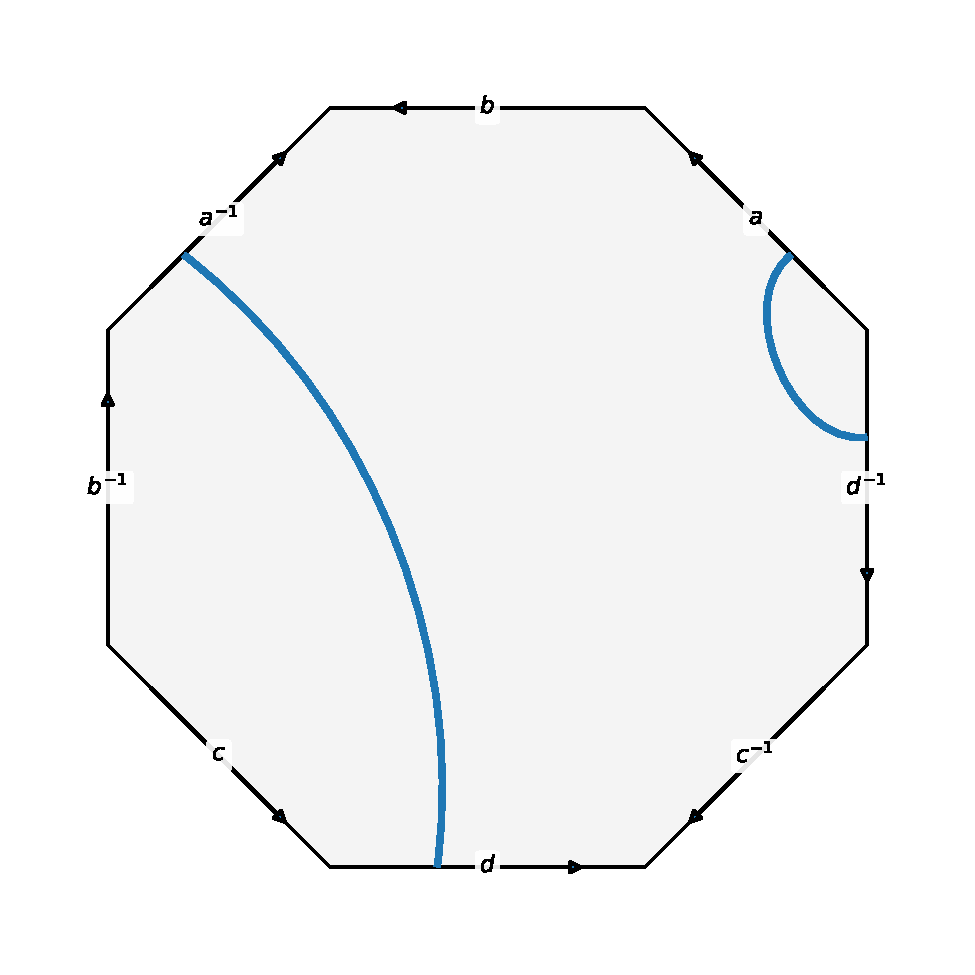
\includegraphics[width=.6\linewidth]{genus2_octagon_two_arcs.pdf}
\end{center}
\ep

\bp There are only finitely many surfaces that admit an embedding of a $3$ regular graph in which every face is a hexagon. 
\begin{enumerate}[label=(\alph*)]
  \item Which are they?
  \item Pick one and draw an embedding of a $3$ regular graph in which every face is a hexagon.
\end{enumerate}
\ep

\bp A compactification of a space $X$ is an embedding of $X$ as a dense subset of a compact Hausdorff space.  You can make a category out of compactifications of $X$ by letting the objects be compactifications with morphisms defined as follows:  a morphism from a compactifaction $f_1:X \to K_1$ to a compactification $f_2:X \to K_2$ is a map $g:K_1 \to K_2$ so that $gf_1=f_2$
\[
\begin{tikzcd}[row sep=2.2em, column sep=3.2em]
 & K_1 \arrow[dd,"g"] \\
 X \arrow[ur,"f_1"] \arrow[dr,swap,"f_2"] \\
& K_2
\end{tikzcd}
\]

Prove that the category of compactifications of $X$ is \emph{thin} meaning that there is at most one morphism between any two compactifications.
\ep

% \bp Let $f:X\to Y$ be a function. 
% \begin{enumerate}[label=(\alph*)]
%   \item Prove that if $U$ is an ultrafilter on $X$ then the pushforward filter $f_*U$ is an ultrafilter on $Y$.
%   \item Now suppose that $X$ and $Y$ are topological spaces.  Prove that $f$ is continuous iff for every ultrafilter $U$ with $U\to x$, the pushforward $f_*(U)\to f(x)$.
% \end{enumerate}
% \ep

\end{document}